\documentclass{article}
\usepackage[T2A]{fontenc}
\usepackage[russian]{babel}
\usepackage[utf8]{inputenc}

%%%%%%%%%%%%%%%%%%%%%%%%%%%% ДОП.СИМВОЛЫ  %%%%%%%%%%%%%%%%%%%%%%%%%%%%%%%%
\usepackage{amsmath}
\usepackage{amssymb}
\usepackage{latexsym}
\usepackage{amsfonts}
\usepackage{extarrows}
\usepackage{braket}
\usepackage{MnSymbol}
\usepackage{mathtools}
\usepackage{commath}

\DeclarePairedDelimiter{\ceil}{\lceil}{\rceil}
\DeclarePairedDelimiter{\floor}{\lfloor}{\rfloor}
%%%%%%%%%%%%%%%%%%%%%%%%%%%%%%%%%%%%%%%%%%%%%%%%%%%%%%%%%%%%%%%%%%%%%%%%

%%%%%%%%%%%%%%%%%%%%%%%%%%%%%  ГРАФИКА  %%%%%%%%%%%%%%%%%%%%%%%%%%%%%%%%
%Цвета:
\usepackage{color} 
\usepackage{xcolor}

%Картиночки:
\usepackage{graphicx}
\graphicspath{{pictures/}}
\DeclareGraphicsExtensions{.pdf,.png,.jpg}

%Встроенная графика 
\usepackage{tikz}
\usetikzlibrary{
    shapes.symbols,
    shapes.geometric,
    shadows,arrows.meta,
    graphs
}

\usepackage{flowchart}
%%%%%%%%%%%%%%%%%%%%%%%%%%%%%%%%%%%%%%%%%%%%%%%%%%%%%%%%%%%%%%%%%%%%%%%%

%%%%%%%%%%%%%%%%%%%%%%%%%%%%%% ВЕРСТКА 1 %%%%%%%%%%%%%%%%%%%%%%%%%%%%%%%%%
\usepackage[toc,page]{appendix}
\usepackage{hyperref}
\hypersetup{
    unicode=true,
    colorlinks=true,
    linktoc=all,  
    linkcolor=blue,
}
\usepackage{hhline}
\usepackage{subcaption}
\usepackage{float}
\usepackage{enumitem}
%%%%%%%%%%%%%%%%%%%%%%%%%%%%%%%%%%%%%%%%%%%%%%%%%%%%%%%%%%%%%%%%%%%%%%%%

%%%%%%%%%%%%%%%%%%%%%%%%%%%%%% ВЕРСТКА 2 %%%%%%%%%%%%%%%%%%%%%%%%%%%%%%%%%
% Шрифты - настройки по умолчанию.
\renewcommand{\rmdefault}{cmr}
\renewcommand{\sfdefault}{cmss}
\renewcommand{\ttdefault}{cmtt}

%Формат секции
\makeatletter
\renewcommand{\@seccntformat}[1]{}
\makeatother


%Пробел
\setlength{\parindent}{0pt}
\setlength{\parskip}{3pt}

%Размеры страницы (не забыть подогнать под принтер)
\usepackage[left=2cm,right=2cm,bottom=2cm]{geometry}

%Списки:
\setlist{topsep=1pt, itemsep=0em}
%%%%%%%%%%%%%%%%%%%%%%%%%%%%%%%%%%%%%%%%%%%%%%%%%%%%%%%%%%%%%%%%%%%%%%%%%%%%%%%%%%%%%%%%%%%%

\title{Чекпоинт II}
\author{Stardust Crusaders}
\date{22 ноября 2020 г.}
\begin{document}
\maketitle
\tableofcontents

\section*{Резюме}
Почти полностью написали реализации моделей. Немного отстаем от плана. Получили первые результаты

\newpage
\section{Цели чекпоинта}
По результатам первого чекпоинта были предложены такие цели:
\begin{itemize}
    \item протестировать предложенные модели;
    \item собрать случайную выборку (с ручной разметкой) для тестирования;
    \item сделать заготовку презентации.
\end{itemize}

Однако, протестировать модели не удалось, так как они не были до конца подготовлены. 

\section{Результаты}

\texttt{Основной github}: \href{https://github.com/Desiment/safety-barriers}{ссылка} 

\texttt{Обработанные данные}: \href{https://drive.google.com/drive/folders/1XhPnQkAMY1KkejASQoEDTFzi1GouzvbE?usp=sharing}{ссылка} 

Сделан заготовок презентации.
Был написан модуль \texttt{prepare}, обрабатывающий сырые данные:
\begin{itemize}
    \item строится очищенная (от цифр и символов пунктуации) таблица. Все слова приводятся в нормальную форму;
    \item строится корпус на основе очищенных данных для \texttt{Word2Vec};
    \item строится словарь уникальных слов, считается частота каждого слова.
\end{itemize}

\begin{figure}[h!]
    \centering
    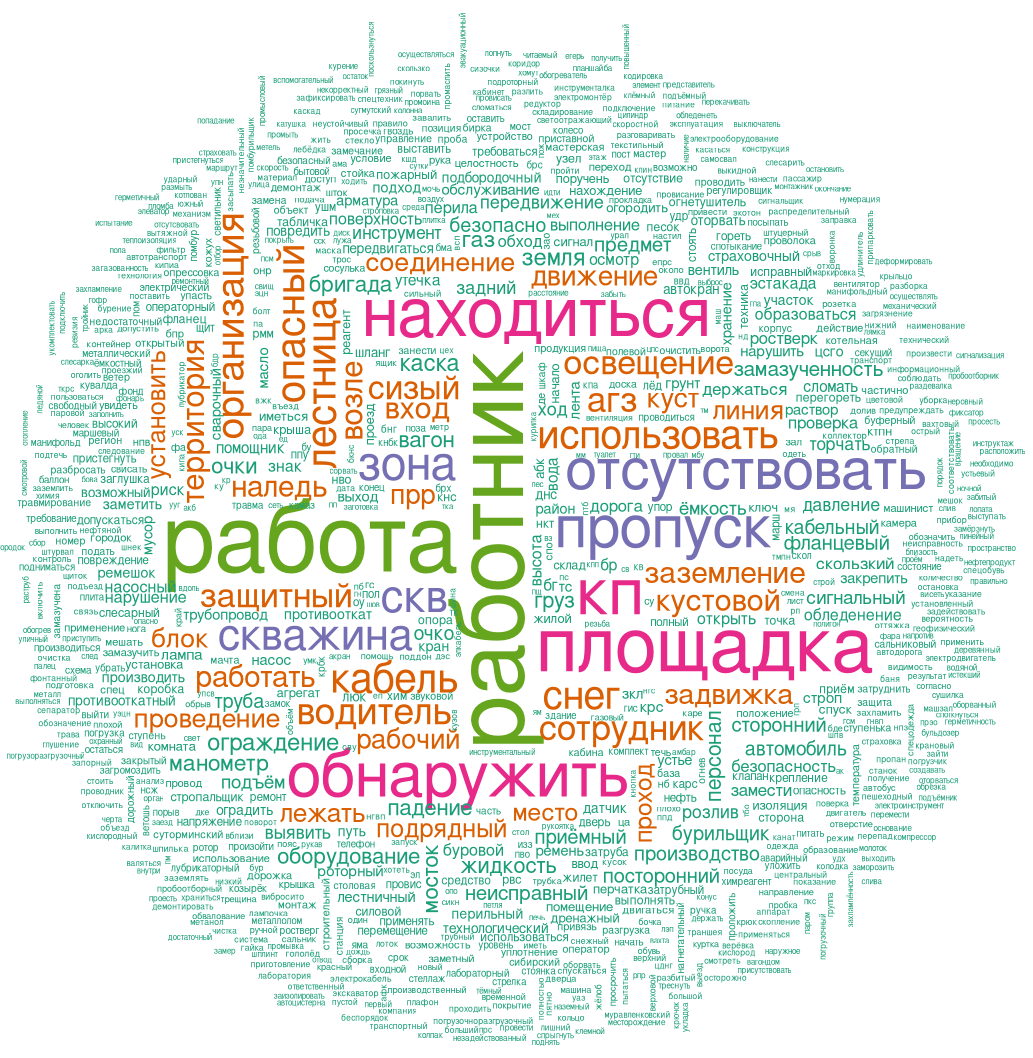
\includegraphics[scale=0.2]{image.png}
    \caption{Облако слов для очищенных данных, построенное с помощью языка R}
\end{figure}

В разработке (написаны, но еще не смердженные в основную ветку) находятся сами модели:

\subsection{Ручная кластеризация}
Каждому кластеру сопоставляется набор ключевых слов в нормальной форме (этот набор выделяется вручную, на основе частности слов)
\begin{enumerate}
    \item Приводим все слова в сообщении в нормальную форму, избавляемся от стопслов и символов пунктуации. 
    \item Проверяем, сколько ключевых слов относящихся к первому кластеру содержится, сколько ко второму и т.д. 
    \item На основе полученных чисел вычисляем кластер объекта:
    \begin{itemize}
        \item В случае, когда есть явный максимум по количеству совпадений, назначаем кластер соответствующий максимуму
        \item В случае, когда ключевых слов практически нет, назначаем кластер ``Другое``.
        \item В случае отсутствия явных совпадений, считаем что оператор указал более одного инцидента в сообщении. 
    \end{itemize}
\end{enumerate}

На данный момент построен классификатор, однако наборы признаков все еще выделяются. 

\subsection{Word2Vec и K-means}
Были построены две реализации этой модели: первая на системе \texttt{KNIME}, вторая была написана на \texttt{Python} с 
использованием библиотеки \texttt{nltk}.

В отличие от предыдущей модели, эта модель не такая прозрачная, но зато полностью автоматизированная. 

\section{Цели на последний чекпоинт}
\begin{itemize}
    \item Доделать презентацию
    \item Протестировать модели
    \item Отрефакторить код моделей
    \item Написать bash-оболочку и документацию
\end{itemize}
\end{document}
